
\documentclass[12pt,a4paper]{article}
\usepackage{graphicx,amssymb, amstext, amsmath, epstopdf, booktabs, verbatim, gensymb, geometry, appendix, natbib, lmodern}
\geometry{letterpaper}

%*************************************
% A latex package for the preparation of tenure and promotion dossier.
% M.R. Hadizadeh
% E-mail: mhadizadeh@gmail.com
% August 2021
%*************************************

\usepackage{latex_style/CSU} % latex style file
\usepackage{url}
 \usepackage{hyperref}
\hypersetup{
    bookmarks=true,         % show bookmarks bar?
    unicode=true,          % non-Latin characters in Acrobat’s bookmarks
    pdftoolbar=true,        % show Acrobat’s toolbar?
    pdfmenubar=true,        % show Acrobat’s menu?
    pdffitwindow=true,     % window fit to page when opened
    pdfstartview={FitH},    % fits the width of the page to the window
    pdftitle={My title},    % title
    pdfauthor={Author},     % author
    pdfsubject={Subject},   % subject of the document
    pdfcreator={Creator},   % creator of the document
    pdfproducer={Producer}, % producer of the document
    pdfkeywords={keyword1} {key2} {key3}, % list of keywords
    pdfnewwindow=true,      % links in new window
    colorlinks=true,       % false: boxed links; true: colored links
    linkcolor=blue,          % color of internal links
    citecolor=blue,        % color of links to bibliography
    filecolor=blue,      % color of file links
    urlcolor=blue,           % color of external links
    pagebackref=yes,
    pdfborder={0 0 100},
    linkbordercolor={0 0 1} 
    }
   
\usepackage[final]{pdfpages}
\usepackage{minibox}
\usepackage[utf8]{inputenc}
\usepackage{fourier}
\usepackage{etaremune}
\usepackage{eqparbox}
\usepackage{fontawesome}
\usepackage{pdfpages}
\usepackage{makecell}
\usepackage{float}
\usepackage{xcolor}
\usepackage[most]{tcolorbox}
\usepackage{lmodern} 
\usepackage{tabu}
\usepackage{array}
\usepackage{colortbl}
\usepackage{multirow}
\usepackage{breakurl}
\usepackage{xltabular}
\usepackage{longtable}
\usepackage{lipsum}
\usepackage[english]{babel}
\usepackage{blindtext}


\newcommand*\cpiType{\leftmark}

%%%%%%%%%%%%%%%%%%% CHANGE HERE %%%%%%%%%%%%%%
\newcommand*\Date{\today}
\newcommand*\Author{FIRSTNAME LASTNAME}
\newcommand*\Authorshort{F. LASTNAME,}
\newcommand*\position{POSITION}
\newcommand*\room{Room \#}
\newcommand*\department{Department NAME}
\newcommand*\college{College NAME}
\newcommand*\university{University NAME}
\newcommand*\citystatezip{CITY, STATE, ZIP Code}
\newcommand*\phone{123 456-7890}
\newcommand*\emialaddress{X @ Y.edu}
\newcommand*\Webaddress{http://www.X.edu/$\sim$Y}
\newcommand*\newrank{Associate Professor}
\newcommand*\Title{\footnotesize Dossier for Tenure and Promotion to \newrank | \Authorshort}
\title{Dossier for Tenure and Promotion to \newrank} 
%%%%%%%%%%%%%%%%%%%%%%%%%%%%%%%%%%%%%%



%%%%%%%%%%
%% header and footer lines
\renewcommand{\footrulewidth}{.2pt} 
\renewcommand{\headrulewidth}{0.2pt}
%%%%%%%%%%
% Changing the title of ToC
\renewcommand{\contentsname}{Table of Contents}
%%%%%%%%%%
%%%%%%%%%%%%%%%%%
% Sections titles
\newcommand{\sectiontitle}[1]
{
\setlength{\fboxsep}{38pt}
\colorbox{csuOrange}{\makebox[8.25in][l]{ \shortstack[l]{\fontsize{26}{30}\rmfamily\color{white} #1   \hfill}}}
}

\newcommand{\sectiontitledouble}[2]
{
\setlength{\fboxsep}{38pt}
\colorbox{csuOrange}{\makebox[10.25in][l]{\shortstack[l]{\fontsize{26}{30}\rmfamily\color{white}  \minibox[]{#1\\ \hskip1.7cm  #2}  \hfill}}}
}
%%%%%%%%%%%%%%%%%

%%%%%%%%%%%%%%%%%%%%%%%%%
% Fake section and subsection to avoid showing the titles
\newcommand{\fakesection}[1]{%
  \par\refstepcounter{section}% Increase section counter
  \sectionmark{#1}% Add section mark (header)
  \addcontentsline{toc}{section}{\protect\numberline{\thesection}#1}% Add section to ToC
  % Add more content here, if needed.
}

\newcommand{\fakesubsection}[1]{%
  \par\refstepcounter{subsection}% Increase subsection counter
  \subsectionmark{#1}% Add subsection mark (header)
  \addcontentsline{toc}{subsection}{\protect\numberline{\thesubsection}#1}% Add subsection to ToC
  % Add more content here, if needed.
}
%%%%%%%%%%%%%%%%%%%%%%%%%

\definecolor{csuOrange}{RGB}{153,0,76}   %{241,85,44}
\definecolor{csuGray}{RGB}{106,100,100}

%%%%%%%%%%%%%%%%%%%
%Fancy Tables
%
\newcolumntype{Y}{>{\raggedleft\arraybackslash}X}
%
\tcbset{tab1/.style={fonttitle=\bfseries\large,fontupper=\normalsize\sffamily,
colback=yellow!10!white,colframe=csuOrange,colbacktitle=red!40!white,
coltitle=black,center title,freelance,frame code={
\foreach \n in {north east,north west,south east,south west}
{\path [fill=csuOrange] (interior.\n) circle (3mm); };},}}
%
\tcbset{tab2/.style={enhanced,fonttitle=\bfseries,fontupper=\normalsize\sffamily,
colback=yellow!10!white,colframe=csuOrange,colbacktitle=red!40!white,
coltitle=black,center title}}
%%%%%%%%%%%%%%%%%%%

%%%%%%%%%%%%%%%%%%%
% Change caption size & color
%\usepackage[font=small]{caption}
\usepackage{caption}
\captionsetup[figure]{font=small}
\captionsetup[table]{labelfont={color=white},font={color=white}}
%%%%%%%%%%%%%%%%%%%

%%%%%%%%%%%%%%%%%%%
% Fonts packages
%\usepackage{lmodern}        % Latin Modern family of fonts. Very much like Computer Modern, but with many more glyphs 
\usepackage[T1]{fontenc}    % fontenc is oriented to output, that is, what fonts to use for printing characters. 
%\usepackage{textcomp}     % required for special glyphs
%\usepackage{fouriernc}
\usepackage{newpxtext}


%%%%%%%%%
% items in Table
\newcommand{\tabitem}{~~\llap{\textbullet}~~}
\usepackage{tabularx}
%%%%%%%%

\makeatletter
\def\input@path{{sections/}{files/}}
%%%% footer setting
\renewcommand{\sectionmark}[1]{%
  \markboth{\ifnum \c@secnumdepth>\z@
      \thesection\hskip 1em\relax
    \fi #1}{}}
\makeatother

\date{\today}
%-----------------------------------------------------------



\begin{document}

\begin{titlepage}
\maketitle
\end{titlepage}

\linespread{1.15} %Set standard document linespacing

\tableofcontents

\newpage

% sections
\newpage
\sectiontitle{1.) Letter of Request}
\fakesection{Letter of Request}

%Address the letter to your Department Chairperson, Library Director, or Associate Research Director and specify exactly what you want to be considered for (i.e. promotion, tenure, or both) and your area(s) of excellence.


\newpage


\includepdf[scale=0.9,pages=1-,pagecommand={}]{Files/1_Request_letter/Request_Letter.pdf}

\newpage
\sectiontitle{2.) Evidence of Eligibility to Apply}
\fakesection{Evidence of Eligibility to Apply}


%(A). Non-Tenured Faculty. Copy of Initial Employment Contract. The initial employment contract will indicate exactly when a candidate was first employed by the University and the years of prior service he or she has been granted. This information will allow the committee to verify the candidate’s eligibility for promotion and/or tenure. The copy of the initial contract of employment need not include the candidate’s salary.
%(B). Tenured Faculty. Evidence of Initial Date of Promotion (For faculty who have received a promotion and/or tenure at CSU): Document the effective date of the new rank by including the first contract at that rank. This documentation may include the letter from the University President stating the date the promotion was granted by the Board of Trustees as per Article 15.26 of the CSU-AAUP contract or a Personnel Action Form (PAF) that verifies the promotion.
%(C). Faculty not on tenure-track are not eligible for promotion or tenure.


\frame{
\textbf{Enclosed Files}

\begin{itemize}
\item Letter of Eligibility for Tenure -- Dated MONTH DAY, YEAR.
\item A copy of PAF, Dated MONTH DAY, YEAR.

\end{itemize}

}


\newpage


\includepdf[scale=0.9,pages=1-,pagecommand={}]{Files/2_Eligibility_letter/Eligibility_letter.pdf}
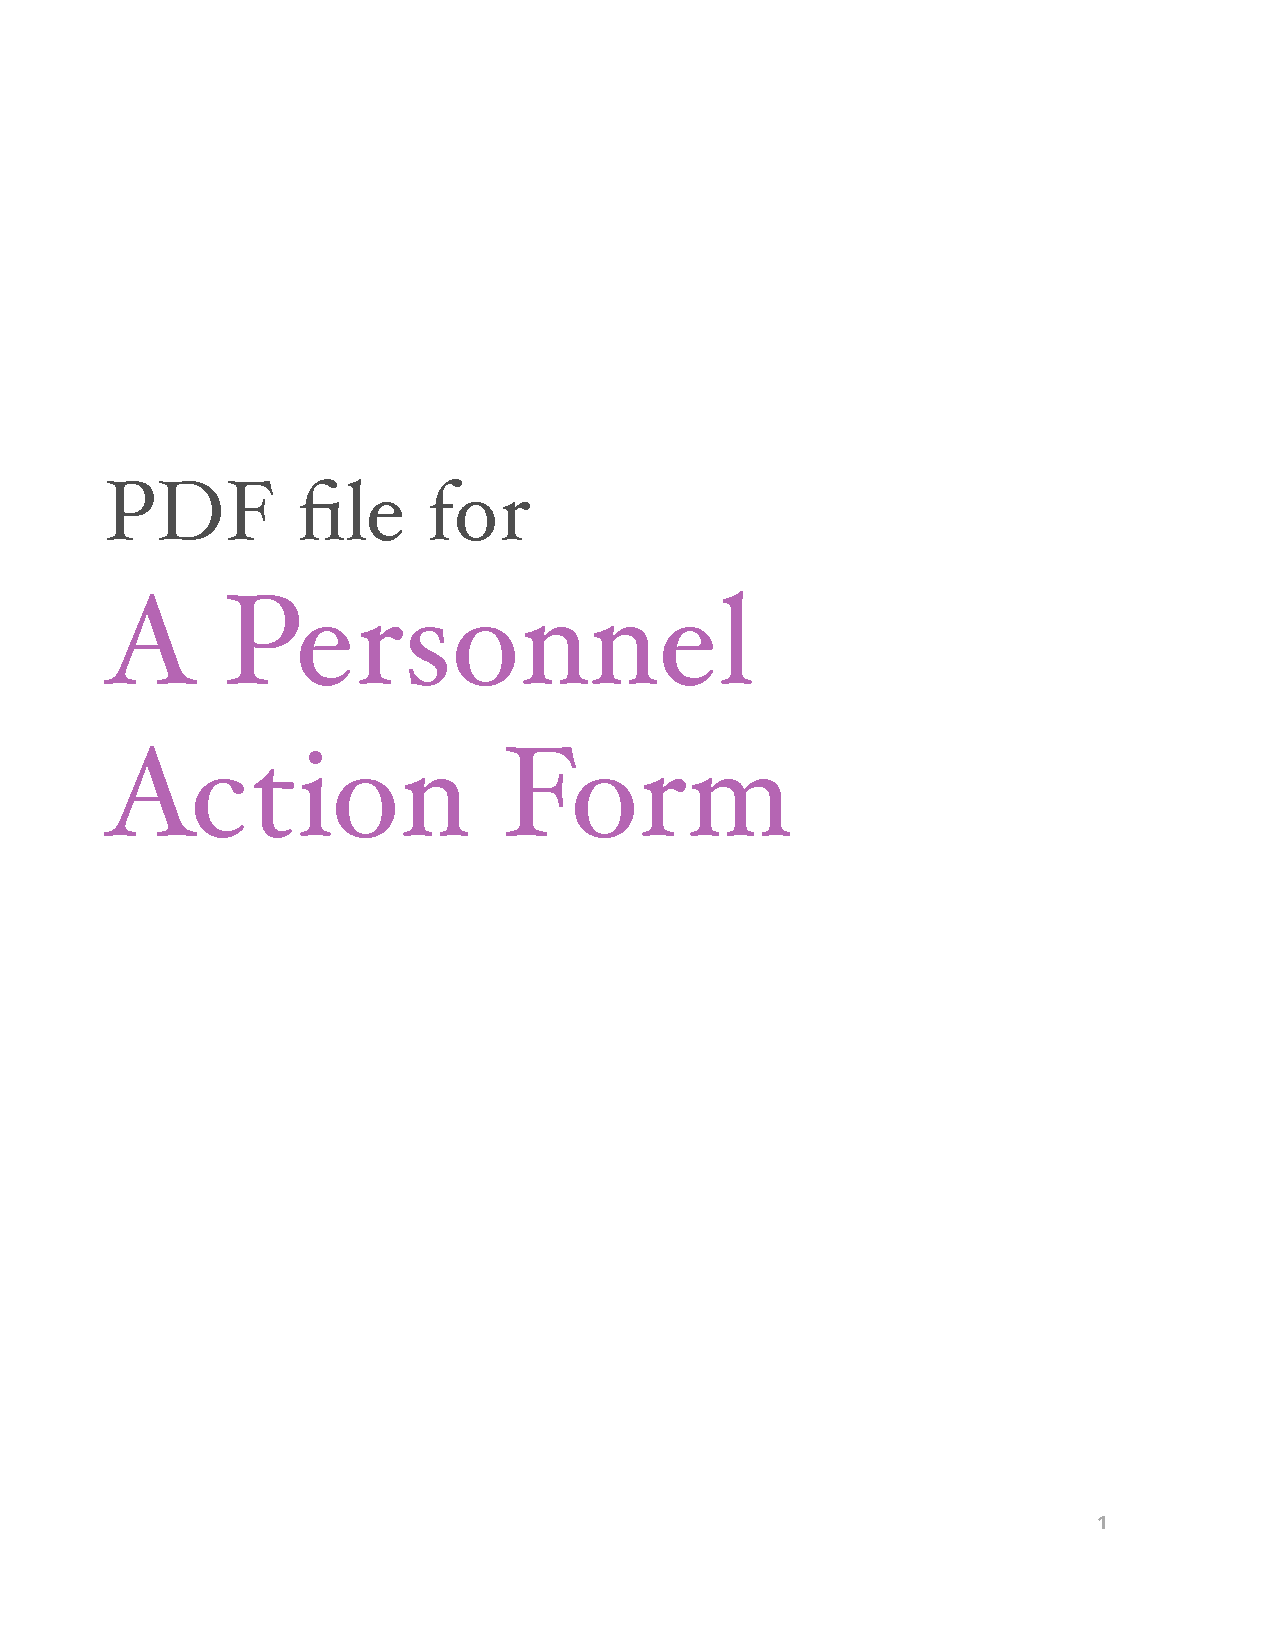
\includepdf[scale=0.9,pages=1-,pagecommand={}]{Files/2_Eligibility_letter/PAF.pdf}


\newpage
\sectiontitle{3.) Curriculum Vitae}
\fakesection{Curriculum Vitae}

%Please include address, email, and phone number at which you can be contacted. At minimum, the curriculum vita should include the following:
%i. Personal information (name, address, e-mail, phone number);
%ii. Education (degrees, certifications, licensures);
%iii. Scholarly publications and presentations funded by state, national, or private grants;
%iv. Teaching experience at CSU and other institutions, academic rank, part time/full time appointments, and dates of teaching service;
%v. Service directly related to the University and dates of service.


\newpage

\includepdf[scale=0.9,pages=1-,pagecommand={}]{Files/3_CV/CV.pdf}

\newpage
\sectiontitledouble{4.) Qualitative Assessment}{by the Faculty Member}
\fakesection{Qualitative Assessment by the Faculty Member}

%Candidates for tenure and promotion should prepare a statement that reflects their own assessment of their teaching, research/creative achievement, and service. Identify any accomplishments associated with or resulting from teaching, research/creative achievement, and service. This statement is the place for the candidate to provide informative commentary on the criteria for promotion and tenure and his or her assessment on how the criteria have been achieved. The assessment should indicate the impact, significance, or value of the work. Candidates should provide clear and sufficient information about their individual roles in collaborative projects, publications, presentations, or grants. In addition, the statement should include specific plans for continuation of the candidate’s research or creative activity agenda, plans to enhance teaching effectiveness, and future participation in service to the University and/or profession. Any service directly provided to external communities must show causal relationship to the University.
%You may use the following questions as a guide.
%Teaching:
%i. How did your teaching develop over the review period?
%ii. Assess the strengths/weaknesses of your teaching and indicate what steps you have taken to improve the quality of the instruction you offer students.
%iii. How has your field changed and how do your courses reflect those changes?
%iv. Whatisespeciallyinnovativeaboutyourcourses?
%v. How do you attend to and measure student learning?
%vi. Howdoyourcoursesplayaroleinachievingdepartmentalorinstitutionalgoals?
%vii. How does your teaching connect to other forms of scholarship?
%viii.What questions do you ask of your own teaching?
%ix. What are your scholarly practices regarding teaching (inquiry, reading, collaboration, revision)?
%x. What texts or theories have influenced the ways you think about your discipline, the students you teach, and the ways you design your courses?
%xi. Howhasnewlearningofyourown(suchasscholarlyinterests,expertisewithtechnology, community engagement) affected your courses and your students’ learning?
%Research:
%i. How did your research/creative activity develop over the review period?
%ii. Assess your research contribution or creative activity with respect to the relevant community (such as scientific community) in general.
%iii. What specific contributions do your research and creative achievements make to your academic discipline?
%iv. How has your research/creative activity helped to benefit you, your department, students, and the institution?
%v. Why do you think your research/creative activity and scholarly work is at the level of your peers in your field of expertise?
%vi. HowdoyouthinkyourgrantshelptoimprovetheUniversity’scapabilities?
%vii. What professional affiliations do you actively engage in membership and how does that contribute to your field or discipline?
%viii.Describe your near future and long-term plans or directions regarding the research/creative activity.
%Service:
%i. Identify University, professional and community groups and/or organizations with which you are working. Describe the nature of the organization(s) and explain your role and/or office within the organization(s).
%ii. Identify your participation in these service organizations and indicate the scope and nature of the efforts.
%iii. What leadership role(s) have you taken in service organizations? What specific accomplishments were achieved under your leadership?
%iv. For University service, describe your responsivity to the institutional needs.
%v. For professional and community service, describe your responsivity to the group’s mission or efforts.
%vi. How have your services benefitted the community and the institution?
%vii. Provide you near future and long term plans or directions with respect to services
%The following sections generally consist of supporting documentation related to teaching, research, and service. External support letters provided as evidence should be from persons who have direct knowledge of candidate’s contribution and can offer verification of the candidate’s qualitative statement.

\newpage

\subsection{Introduction}
\blindtext

\subsection{Research}
\blindtext

\subsection{Teaching}
\blindtext


\begin{quotation}
``{\it \small Here is a sample quotation: \blindtext}''
\end{quotation}

%
\begin{figure}[H]
\caption{Here is a sample figure.}
\centering
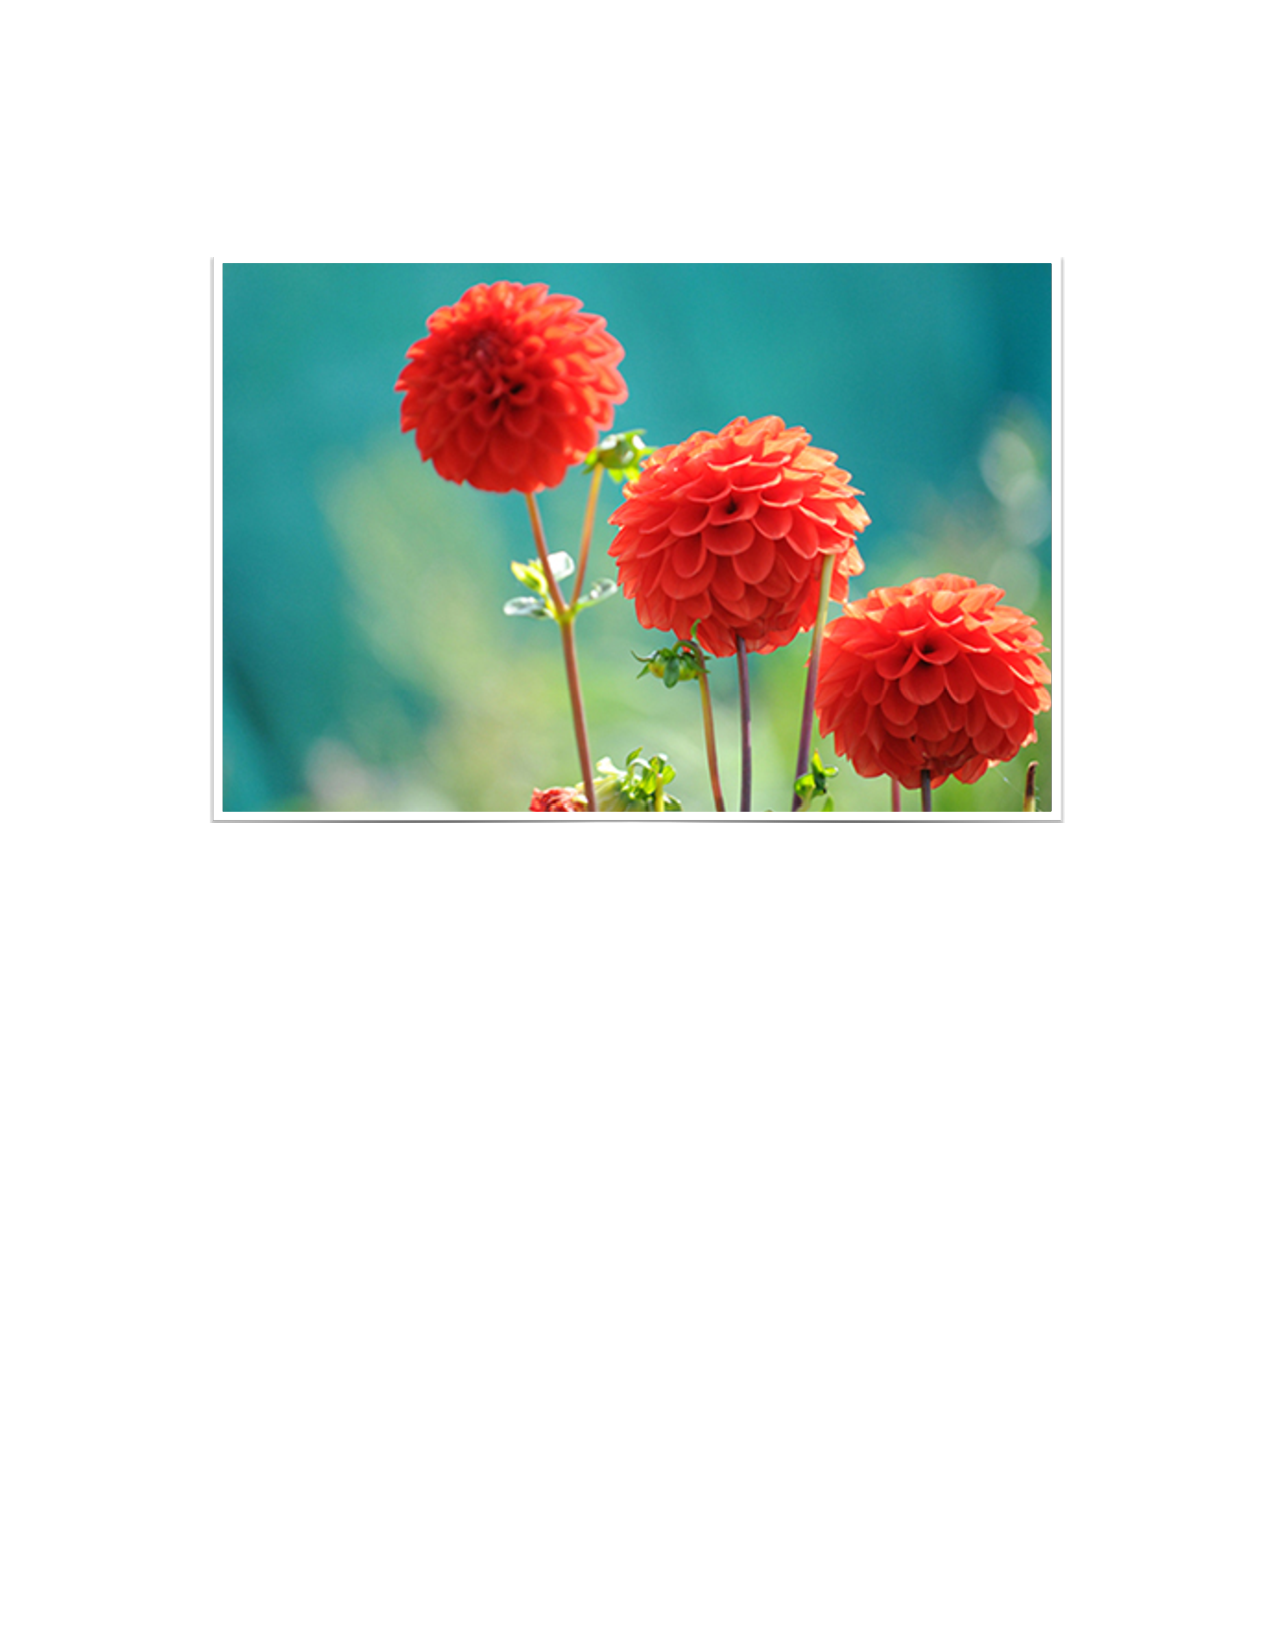
\includegraphics[width=0.5\textwidth]{Files/4_Qualitative_Assessment/Fig.pdf}
\label{fig_label}
\end{figure}




\subsection{Service}
\blindtext


\subsection{Summary}
\blindtext

\newpage
\sectiontitle{5.) Instructional Assignments}
\fakesection{Instructional Assignments}

%List courses taught at CSU. Separately, list courses taught at other schools, including when and where.
%i. Librarianship is equivalent to that of the classroom faculty. Reference service/delivery of information, such as course integrated hands-on active learning, bibliographic instruction, tutorials and research guides, collection development, organization of knowledge, instruction— information literacy, liaison activities, managing student employees, cataloging resources and systems are effective teaching.
%ii. For Research faculty, supervision of undergraduate student research is equivalent to that of classroom faculty. These activities include, but are not limited to, advising student research and mentoring student research publications.
\newpage



\begin{table}[H]
\centering
%\captionof{table}{}
\label{Teaching_assignment}
\begin{tcolorbox}[colback=yellow!10!white,colframe=csuOrange,title=\caption{A complete list of the courses taught by Dr. X.}]
\begin{tcolorbox}[tab2,tabularx={l}]
{\bf University NAME (2016--2020)}  \\
 \toprule
%
Spring 2020 \\
\quad\faCaretRight~ COURSE NAME (COURSE CODE) \\
\quad\faCaretRight~  COURSE NAME (COURSE CODE) \\
%
Fall 2019 \\
\quad\faCaretRight~ COURSE NAME (COURSE CODE) \\
%
Spring 2019 \\
\quad\faCaretRight~ COURSE NAME (COURSE CODE) \\
%
Fall 2018: \\
\quad\faCaretRight~ COURSE NAME (COURSE CODE) \\
%
Spring 2018: \\
\quad\faCaretRight~ COURSE NAME (COURSE CODE) \\
%
Fall 2017: \\
\quad\faCaretRight~ COURSE NAME (COURSE CODE) \\
%
 Spring 2017:  \\
\quad\faCaretRight~ COURSE NAME (COURSE CODE) \\
%
Fall 2016:  \\
\quad\faCaretRight~ COURSE NAME (COURSE CODE) \\
%
  \specialrule{1.5pt}{1pt}{1pt}
%
%
{\bf OTHER University NAME (2015)}  \\
 \midrule
 Fall 2015: \\
\quad\faCaretRight~  COURSE NAME (COURSE CODE) \\
%
\bottomrule
\hskip9.5cm  Continued on next page \faCaretRight\faCaretRight\faCaretRight
    \\
\bottomrule
\end{tcolorbox}
\end{tcolorbox}
\end{table}


\begin{table}[H]
  \centering
\begin{tcolorbox}[colback=yellow!10!white,colframe=csuOrange,title=\caption*{
  Table 1 -- continued from previous page.}]
\begin{tcolorbox}[tab2,tabularx={l}] %{X||Y|Y|Y|}
{\bf OTHER University NAME (2004--2009)}  \\
 \toprule
%
Spring 2009:  \\
\quad\faCaretRight~  COURSE NAME (COURSE CODE) \\
%
Spring 2008:  \\
\quad\faCaretRight~  COURSE NAME (COURSE CODE) \\
%
Fall 2007:  \\
\quad\faCaretRight~  COURSE NAME (COURSE CODE) \\
%
Spring 2006:  \\
\quad\faCaretRight~  COURSE NAME (COURSE CODE) \\
\quad\faCaretRight~  COURSE NAME (COURSE CODE) \\
%
Fall 2005:  \\
\quad\faCaretRight~  COURSE NAME (COURSE CODE) \\
\quad\faCaretRight~  COURSE NAME (COURSE CODE) \\
 %
 Spring 2004:  \\
 \quad\faCaretRight~  COURSE NAME (COURSE CODE) \\
 \quad\faCaretRight~  COURSE NAME (COURSE CODE) \\

  %
%
\bottomrule
\end{tcolorbox}
\end{tcolorbox}
\label{Teaching_assignment_continued}
\end{table}

\newpage
\sectiontitle{6.) Teaching Loads}
\fakesection{Teaching Loads}
\label{Teaching_Load}
 %List contact hours taught for the last six semesters. Include a thorough explanation if your teaching load is significantly above or below the norm. For research and hybrid faculty, assigned supervision of undergraduate student research should also be listed here.

\newpage



\begin{table}[H]
  \centering
\begin{tcolorbox}[colback=yellow!10!white,colframe=csuOrange,title= \caption{
  \textcolor{white}{List of the courses taught by Dr. X in the \underline{last six semesters}.}}]
%\begin{tcolorbox}[tab2,tabularx={c||c|c|c|c|c}] %{X||Y|Y|Y|}
\taburulecolor{csuOrange}
\begin{tabularx}{\linewidth}{ c||c|c|c|c|c }
  \toprule
\multirow{2}{*}{Term} & \multirow{2}{*}{CRN} & \multirow{2}{*}{Course Title} & Credit & \# of  & Teaching/Research    \\
 &  &     & Hours & Enrollment &  Load    \\
\midrule
\midrule
\multirow{2}{*}{Spring 2020}
&  12345   & PHY 1111  & 3   & 15 & \multirow{2}{*}{50/50 \%} \\
&  43210   & PHY 2222  & 5    & 10 \\
\hline
%
\multirow{1}{*}{Fall 2019}
&  12345   & PHY 1111  & 3   & 15 & \multirow{1}{*}{50/50 \%} \\
\bottomrule
%
\multicolumn{6}{c}{Total Credit Hours (2019--2020): 11/12} \\
\bottomrule
%
\multirow{2}{*}{Spring 2019}
&  12345   & PHY 1111  & 3   & 15 & \multirow{2}{*}{50/50 \%} \\
&  43210   & PHY 2222  & 5    & 10 \\
\hline
%
\multirow{1}{*}{Fall 2018}
&  12345   & PHY 1111  & 3   & 15 & \multirow{1}{*}{50/50 \%} \\
\bottomrule
%
\multicolumn{6}{c}{Total Credit Hours (2018--2019): 11/12} \\
\bottomrule
%
\multirow{2}{*}{Spring 2018}
&  12345   & PHY 1111  & 3   & 15 & \multirow{2}{*}{50/50 \%} \\
&  43210   & PHY 2222  & 5    & 10 \\
\hline
%
\multirow{1}{*}{Fall 2017}
&  12345   & PHY 1111  & 3   & 15 & \multirow{1}{*}{50/50 \%} \\
\bottomrule
%
\multicolumn{6}{c}{Total Credit Hours (2017--2018): 11/12} \\
\bottomrule
%
%
\end{tabularx}
%\end{tcolorbox}

\vskip1cm
{\footnotesize
%
\begin{itemize}
\item PHY 1111: COURSE TITLE
\item PHY 2222: COURSE TITLE
\end{itemize}
%
}

\end{tcolorbox}
\end{table}

\newpage
{\bf Justification of lower teaching loads}
\begin{itemize}
\item {\bf Justification 1} \\
\blindtext


\item {\bf Justification 2} \\
\blindtext


\item {\bf Justification 3} \\
\blindtext


\end{itemize}

\newpage
\sectiontitledouble{7.) Evidence in Support of}{Effective Teaching}
\fakesection{Evidence in Support of Effective Teaching}
\newpage
%For the purposes of promotion and tenure, “Effective Teaching” is defined as a demonstration of reflective teaching practices that illustrate the scope and quality of the professor’s teaching. To this end, the promotion and tenure dossier should include a structured reflection of selected information on teaching activities, provide strong evidence of teaching performance, and demonstrate approaches to evaluating teaching for improvement. The emphasis of the dossier should be placed on the strategies that the candidate employs in teaching and an assessment of their effectiveness. Student learning is a combination of both the teacher’s strategies and the students’ effort to process this information. Therefore, DFW rates, which emphasize the student’s effort, should not be taken solely into consideration for the purposes of evaluation of the candidate’s teaching effectiveness.
%At minimum, the dossier should include:
%(A). Teaching Philosophy. Provide a reflective essay about your teaching beliefs and practices. Some aspects you may wish to present include your conception of how learning occurs, description and evidence of how your teaching facilitates student learning, the goals you have for yourself and your students, description of what for you constitutes student learning and the techniques, activities, and methods you use to achieve this goal. Generic philosophical statements about teaching do not fulfill this criterion.
%(B). Evidence of Teaching Methods. Include sample syllabi, course materials, and/or assignments. [Photocopies of up to 10 pages may be included here.]
%(C). Evaluations of Teaching Effectiveness by Students. Please include printouts of course and teacher evaluations. Include here a brief narrative of your interpretation of these evaluations and what they say about you as a teacher. If applicable, include also an explanation of the cause(s) for missing evaluations.

\subsection{Teaching Philosophy}
\label{Teaching_Philosophy}
\blindtext



\subsection{Evidence of Teaching Methods}

In the following, a sample syllabus, slides, and weekly assignment for the {\it COURSE NAME} I taught in SEMESTER YEAR are enclosed.

\newpage


\includepdf[scale=0.9,pages=1-,pagecommand={}]{Files/7_Evidence_in_Support_of_Effective_Teaching/Syllabus.pdf}


\includepdf[scale=0.9,pages=1-,pagecommand={}]{Files/7_Evidence_in_Support_of_Effective_Teaching/Assignment.pdf}

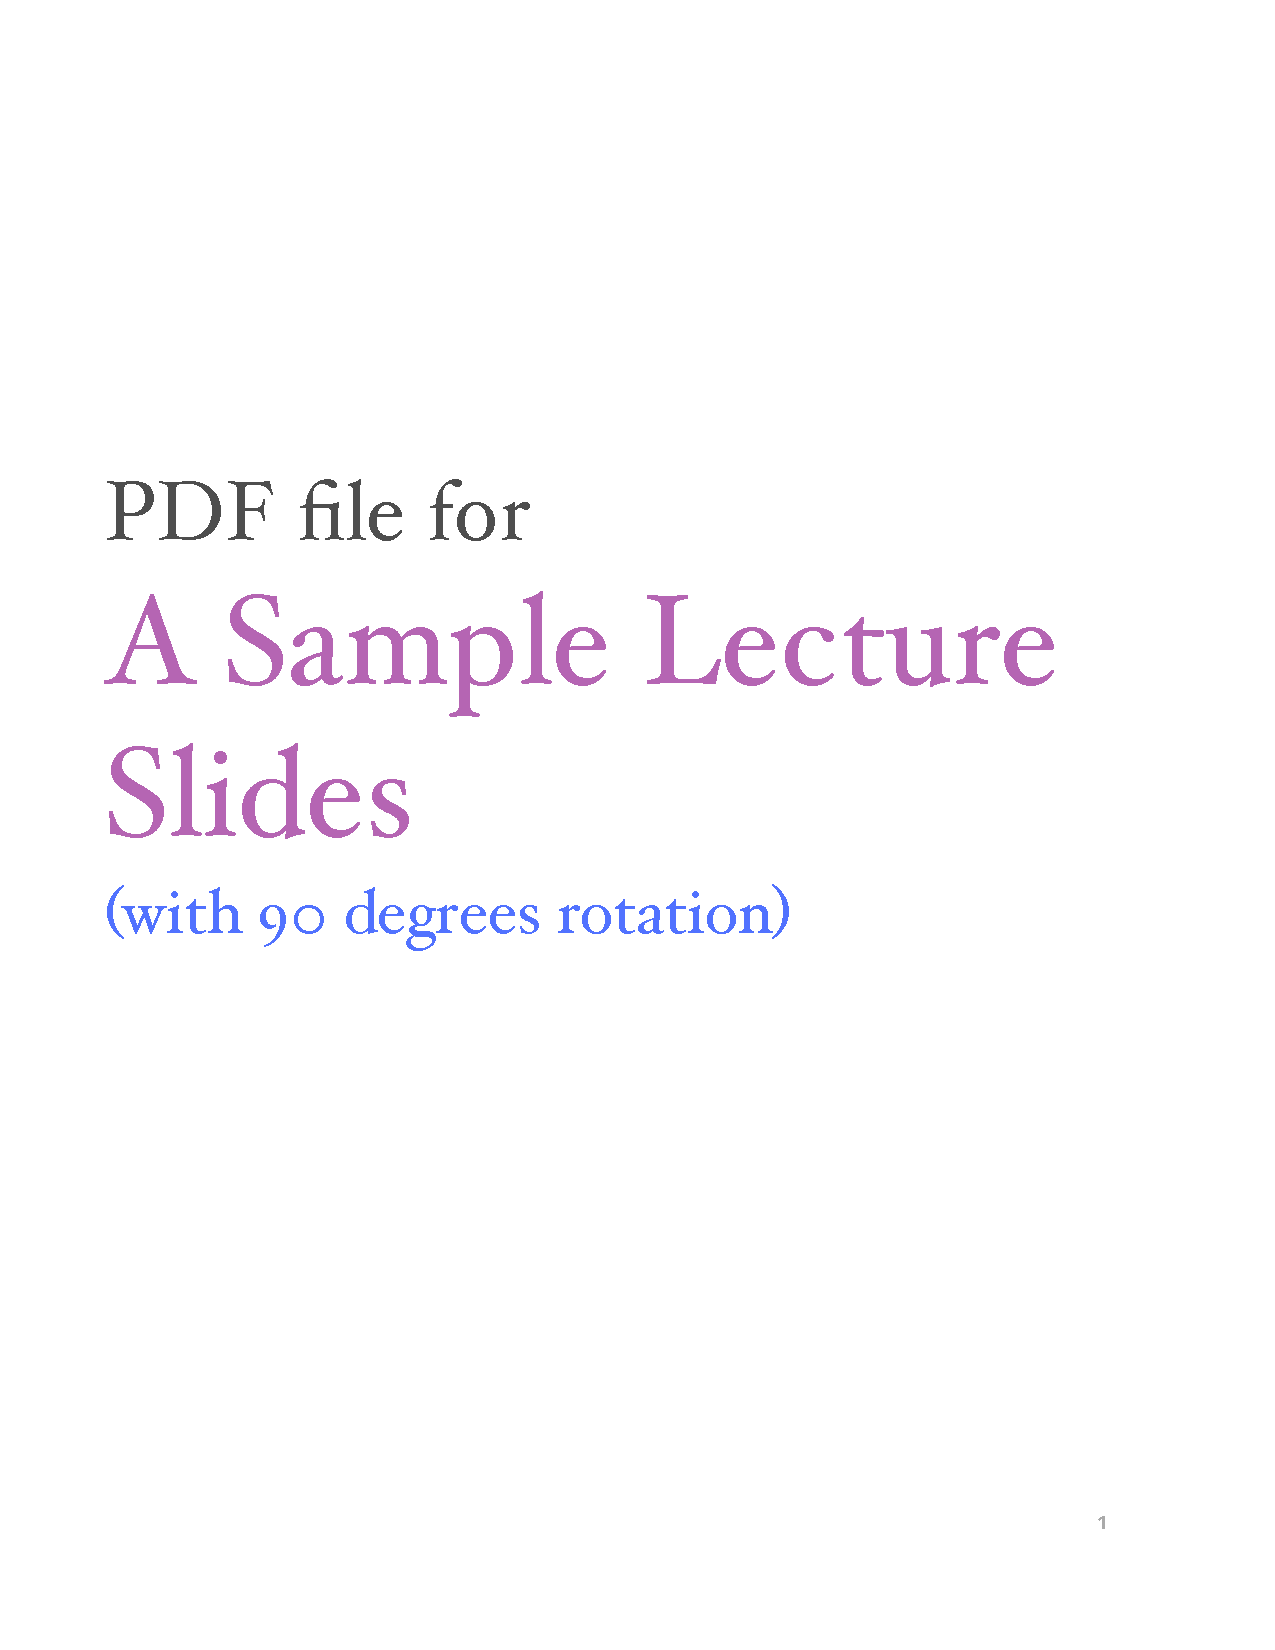
\includepdf[scale=0.9,pages=1-,pagecommand={},angle=90]{Files/7_Evidence_in_Support_of_Effective_Teaching/Lecture.pdf}



\subsection{Evaluations of Teaching Effectiveness by Students}

\blindtext


\begin{table}[H]
  \centering
\begin{tcolorbox}[colback=yellow!10!white,colframe=csuOrange,title= \caption{
  \textcolor{white}{Qualitative feedback from students in the courses taught by Dr. X in the academic year 2019-2020.}}]

\taburulecolor{csuOrange}
\begin{xltabular}{\textwidth}{c | X  | l}

\toprule
Course & Students' Feedback &  \\
%%%%%%%%%%%Spring 2020%%%%%%%%%%%%%%%%
\midrule
%
\multirow{25}{*}{\rotatebox{90}{COURSE NAME}}
& \tabitem

\blindtext

& \multirow{25}{*}{\rotatebox{90}{SEMESTER YEAR}}
\\
& \tabitem
\blindtext
\\
& \tabitem
\blindtext
\\
\bottomrule
  \multicolumn{3}{r}{Continued on next page \faCaretRight\faCaretRight\faCaretRight}  \\
\bottomrule
%%%%%%%%%%%%%%%%%%%%%%%%%%%
\end{xltabular}
\end{tcolorbox}
\label{table_evaluation_2019-2020}
\end{table}

\begin{table}[H]
  \centering
\begin{tcolorbox}[colback=yellow!10!white,colframe=csuOrange,title= \caption*{
  \textcolor{white}{Table 3 -- continued from previous page}}]
\taburulecolor{csuOrange}
\begin{xltabular}{\textwidth}{c | X  | l}
\toprule
Course & Students' Feedback &  \\
%%%%%%%%%%%Fall 2019%%%%%%%%%%%%%%%%
\midrule
%
\multirow{11}{*}{\rotatebox{90}{COURSE NAME}}
& \tabitem
\blindtext
& \multirow{11}{*}{\rotatebox{90}{SEMESTER YEAR}}
\\
\midrule
%
\multirow{24}{*}{\rotatebox{90}{ANOTHER COURSE NAME}}
& \tabitem
\blindtext
& \multirow{24}{*}{\rotatebox{90}{SEMESTER YEAR}}
\\
& \tabitem
\blindtext
\\
& \tabitem
\blindtext
\\
  \bottomrule
%%%%%%%%%%%%%%%%%%%%%%%%%%%
\end{xltabular}
\end{tcolorbox}
\label{table_evaluation_2019-2020_Continued}
\end{table}


\newpage

A copy of the course and instructor evaluations for the courses Dr. X has taught from SEMESTER YEAR to SEMESTER YEAR are enclosed. The following sections did not receive the minimum number of responses required for viewing reports:
\begin{itemize}
\item SEMESTER YEAR: COURSE NAME (SECTION \#): COURSE TITLE [X out of Y Students Responded]

\item SEMESTER YEAR: COURSE NAME (SECTION \#): COURSE TITLE [X out of Y Students Responded]

\end{itemize}

\newpage

% Year 1 evaluations

\includepdf[scale=0.9,pages=1-,pagecommand={},angle=0]{Files/7_Evidence_in_Support_of_Effective_Teaching/Evaluations/Y1/Evaluation1.pdf}
%
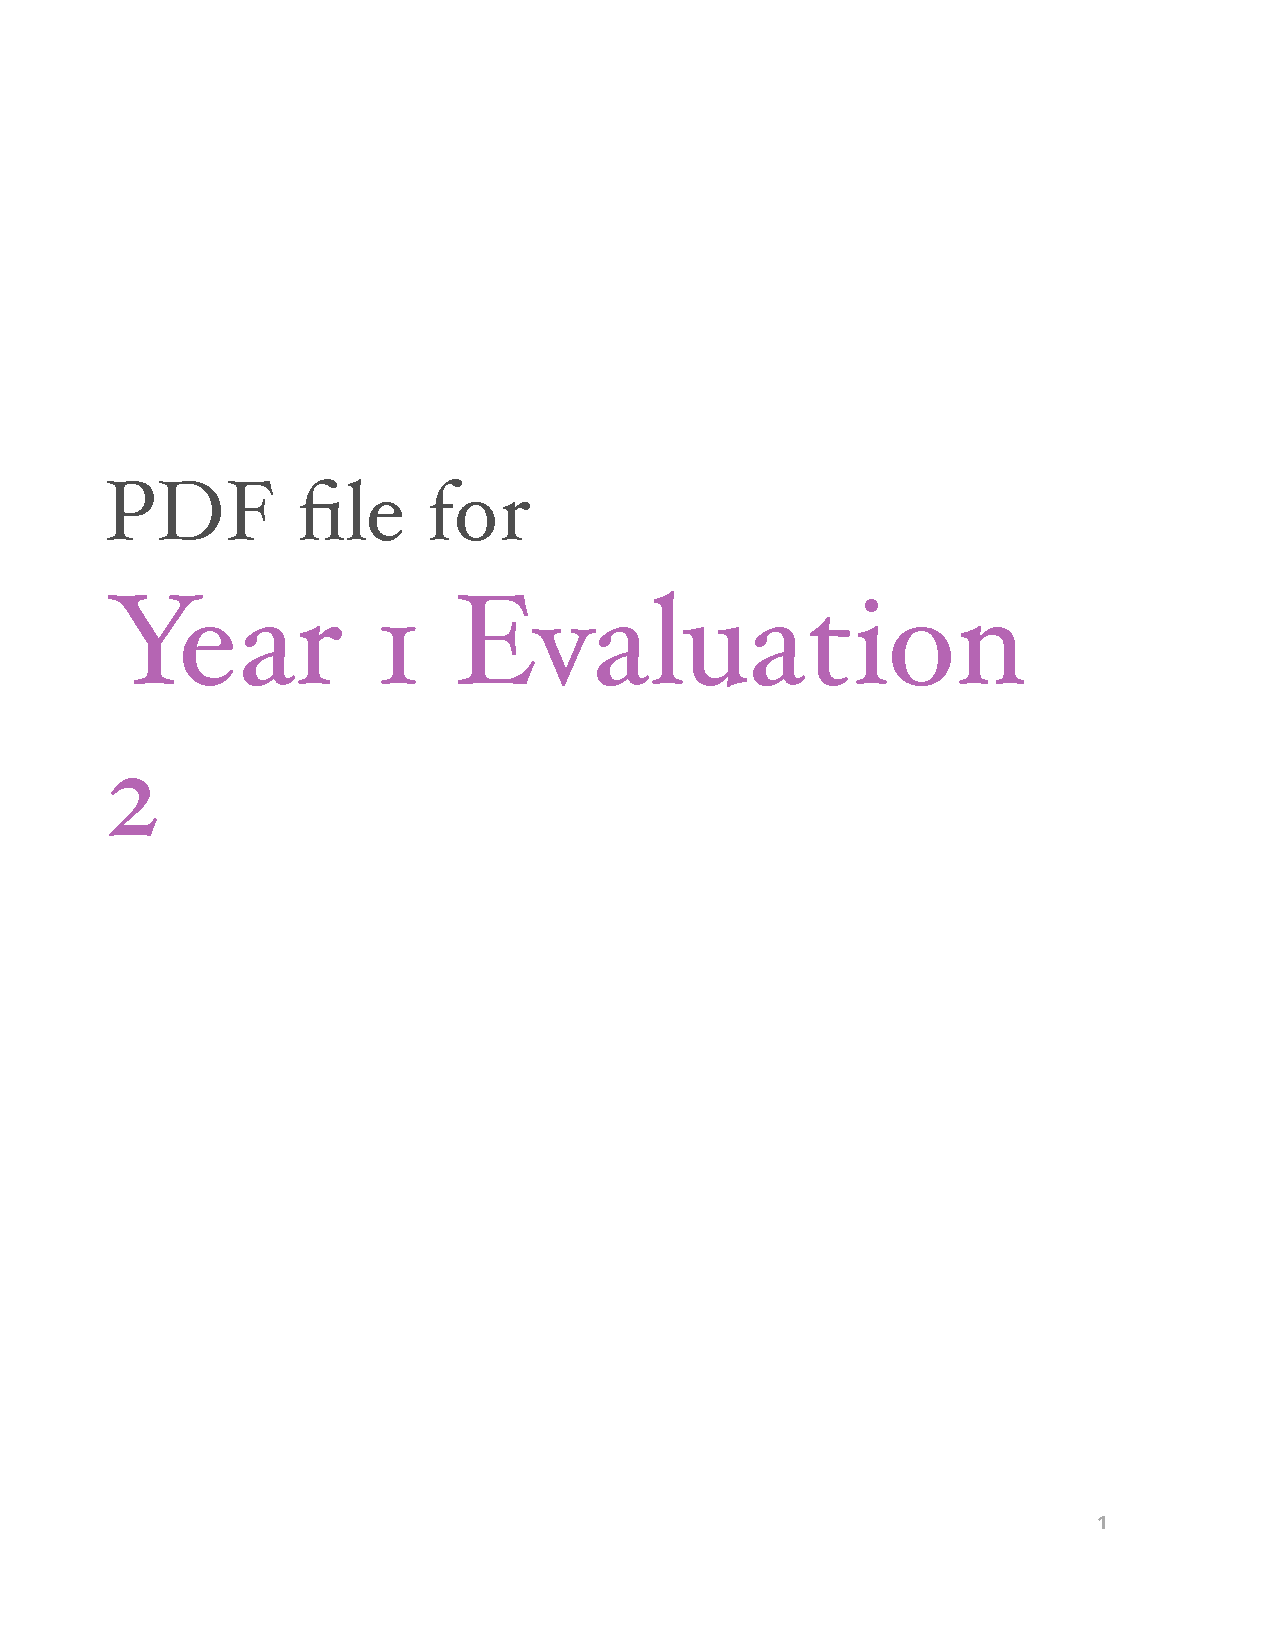
\includepdf[scale=0.9,pages=1-,pagecommand={},angle=0]{Files/7_Evidence_in_Support_of_Effective_Teaching/Evaluations/Y1/Evaluation2.pdf}

% Year 2 evaluations
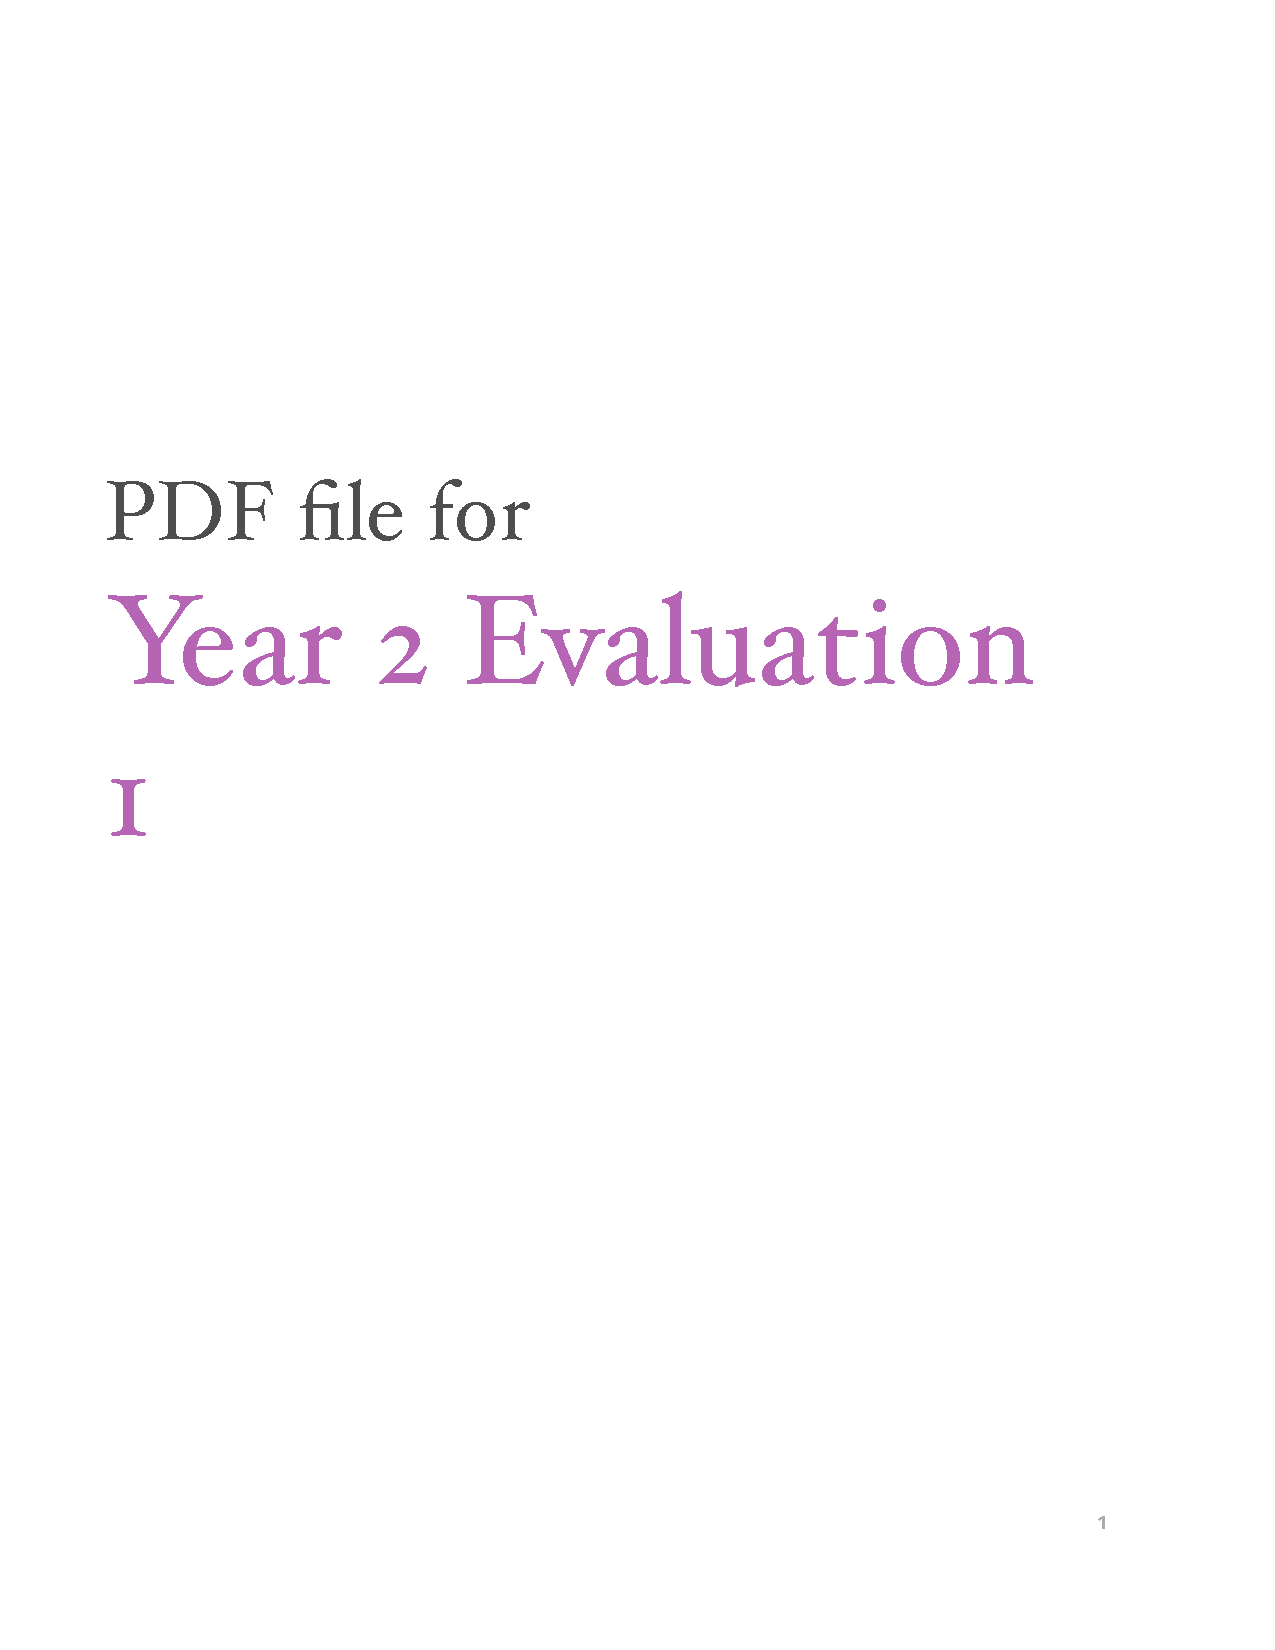
\includepdf[scale=0.9,pages=1-,pagecommand={},angle=0]{Files/7_Evidence_in_Support_of_Effective_Teaching/Evaluations/Y2/Evaluation1.pdf}
%
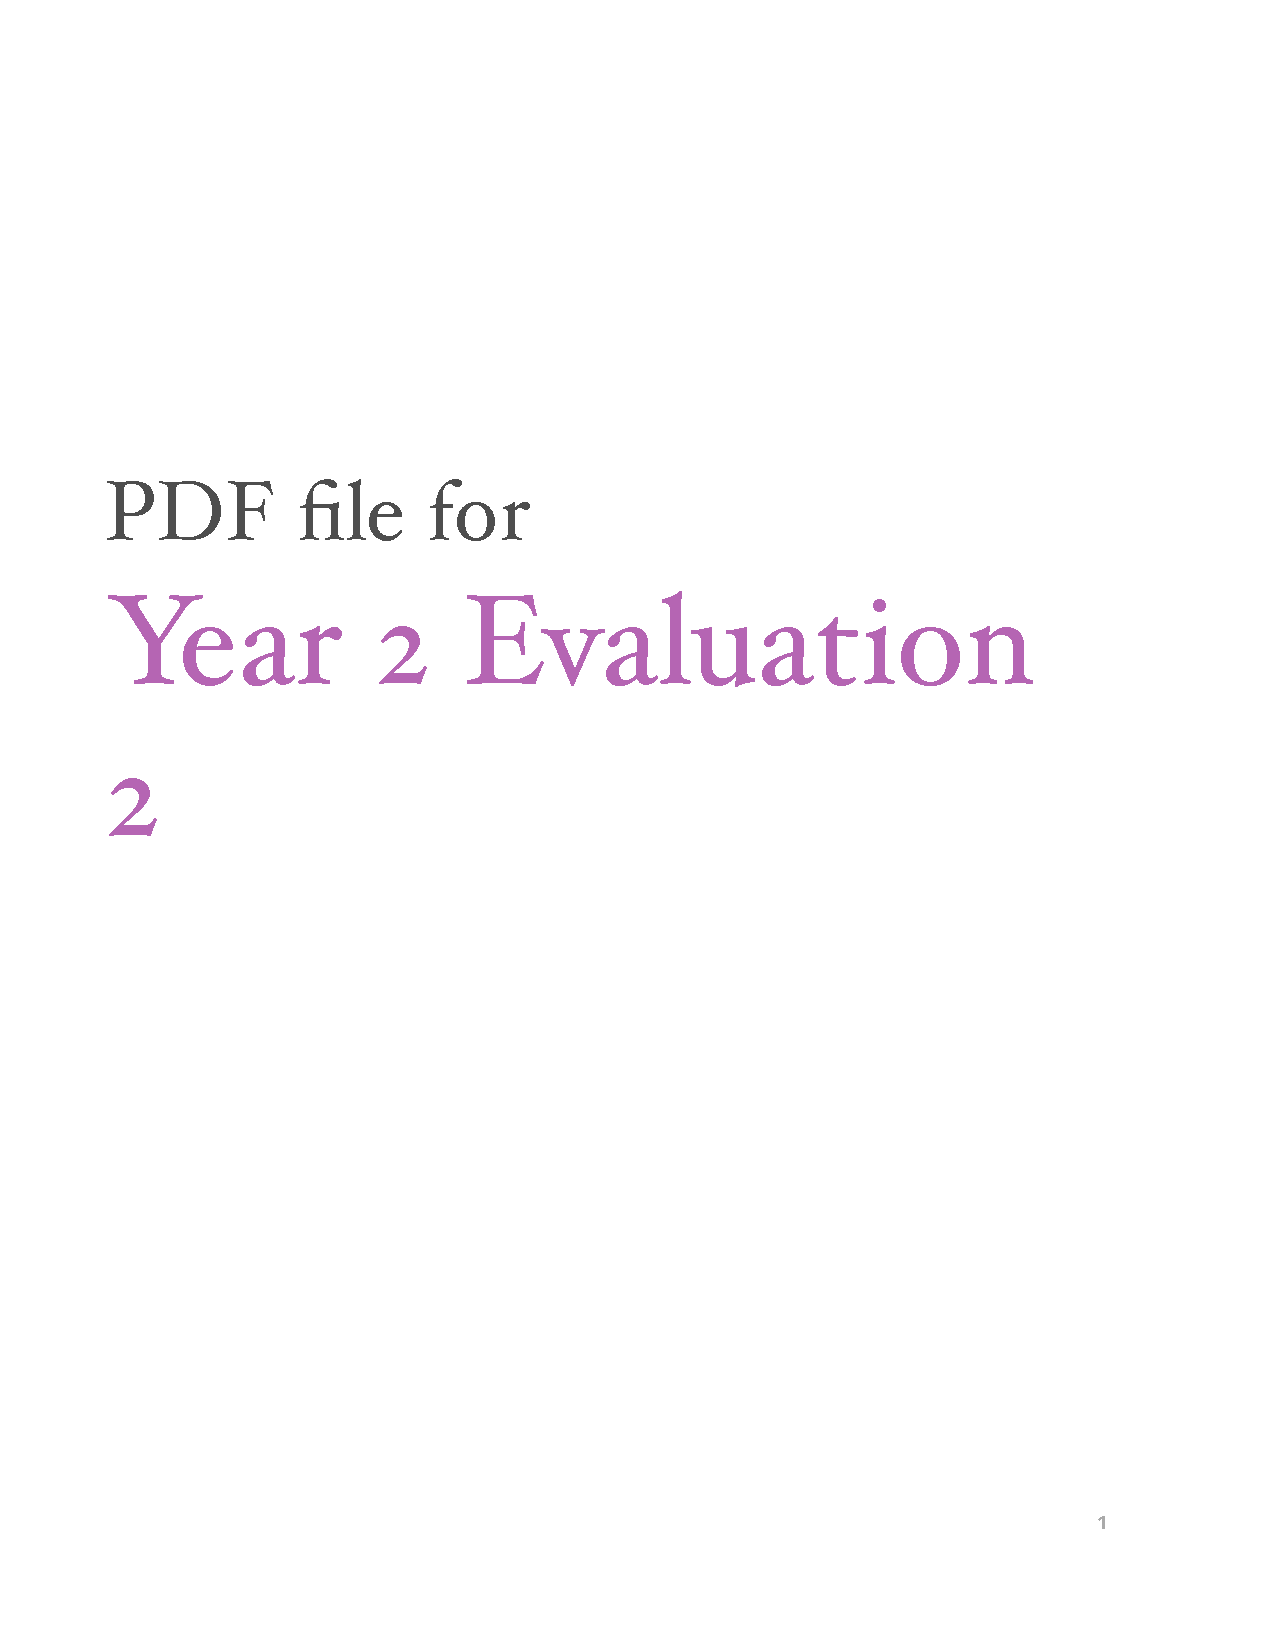
\includepdf[scale=0.9,pages=1-,pagecommand={},angle=0]{Files/7_Evidence_in_Support_of_Effective_Teaching/Evaluations/Y2/Evaluation2.pdf}

% Year 3 evaluations
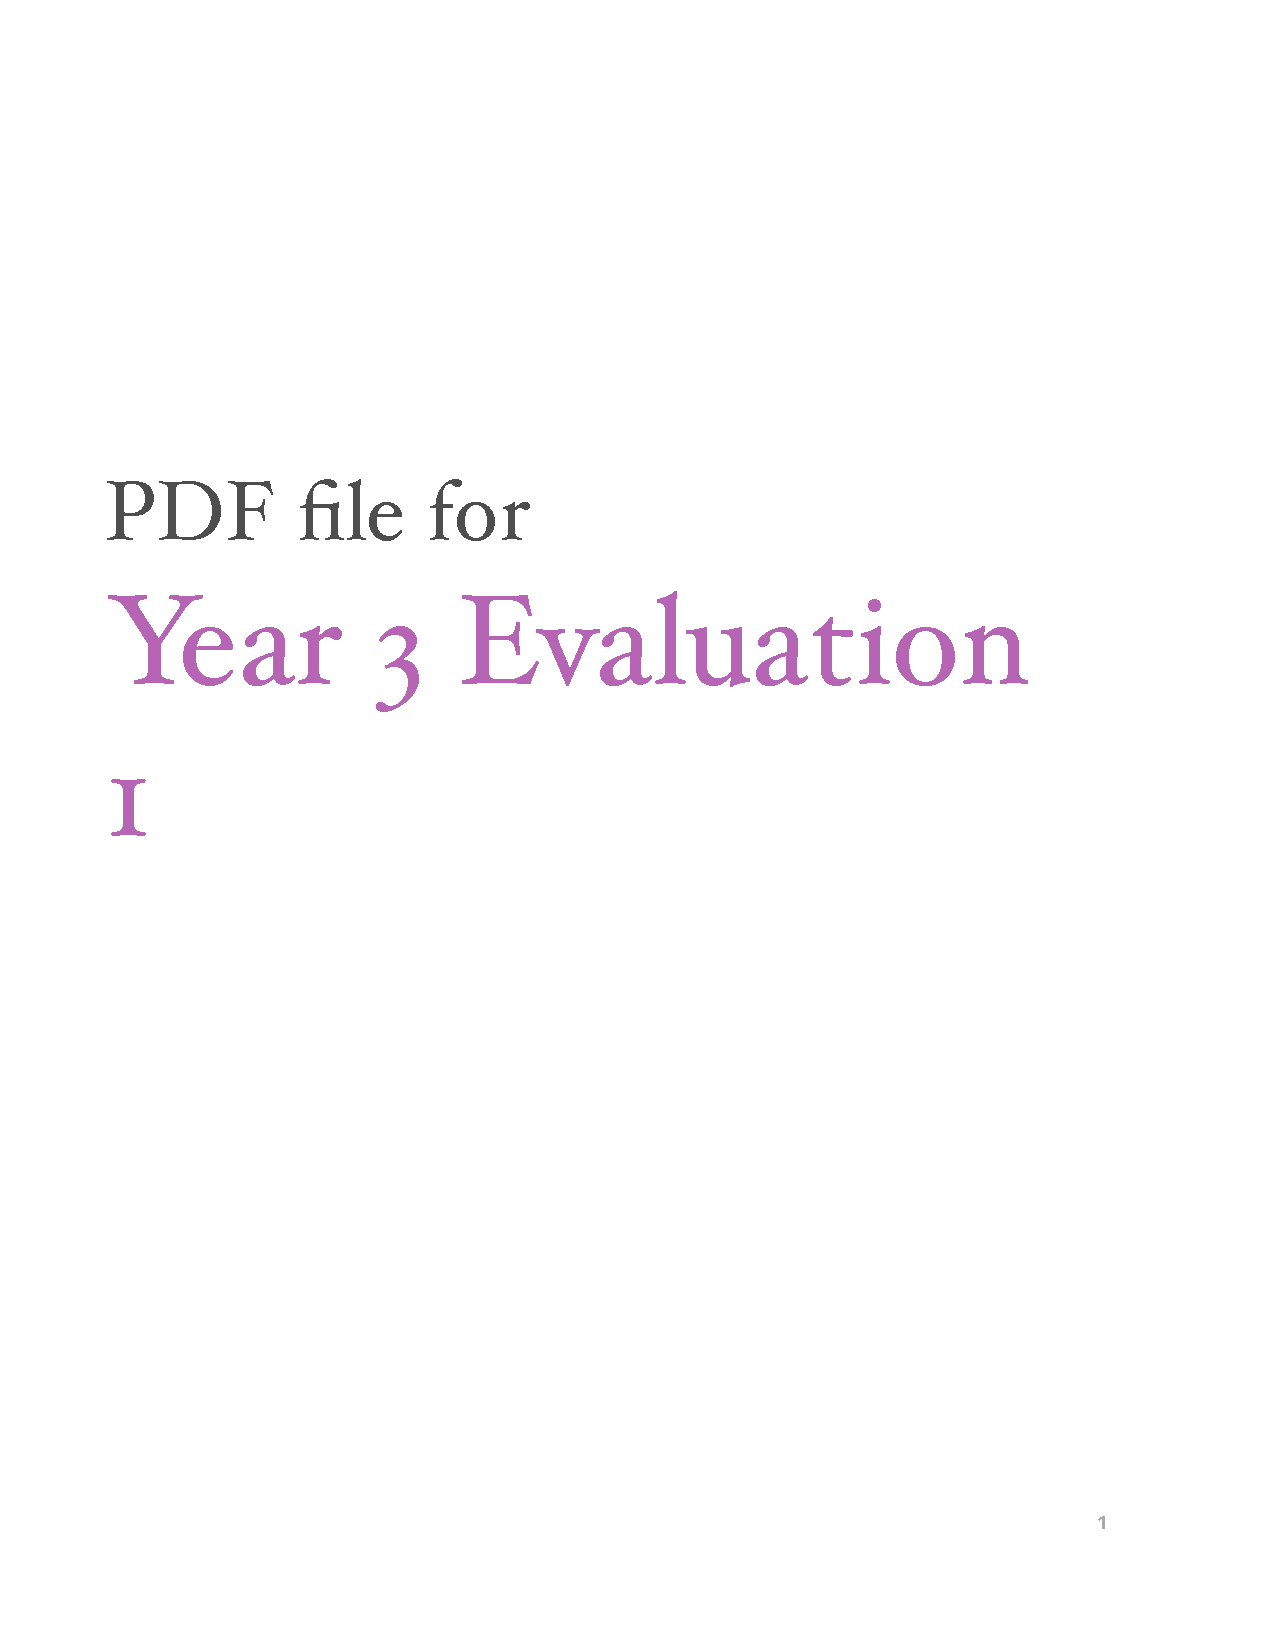
\includepdf[scale=0.9,pages=1-,pagecommand={},angle=0]{Files/7_Evidence_in_Support_of_Effective_Teaching/Evaluations/Y3/Evaluation1.pdf}
%
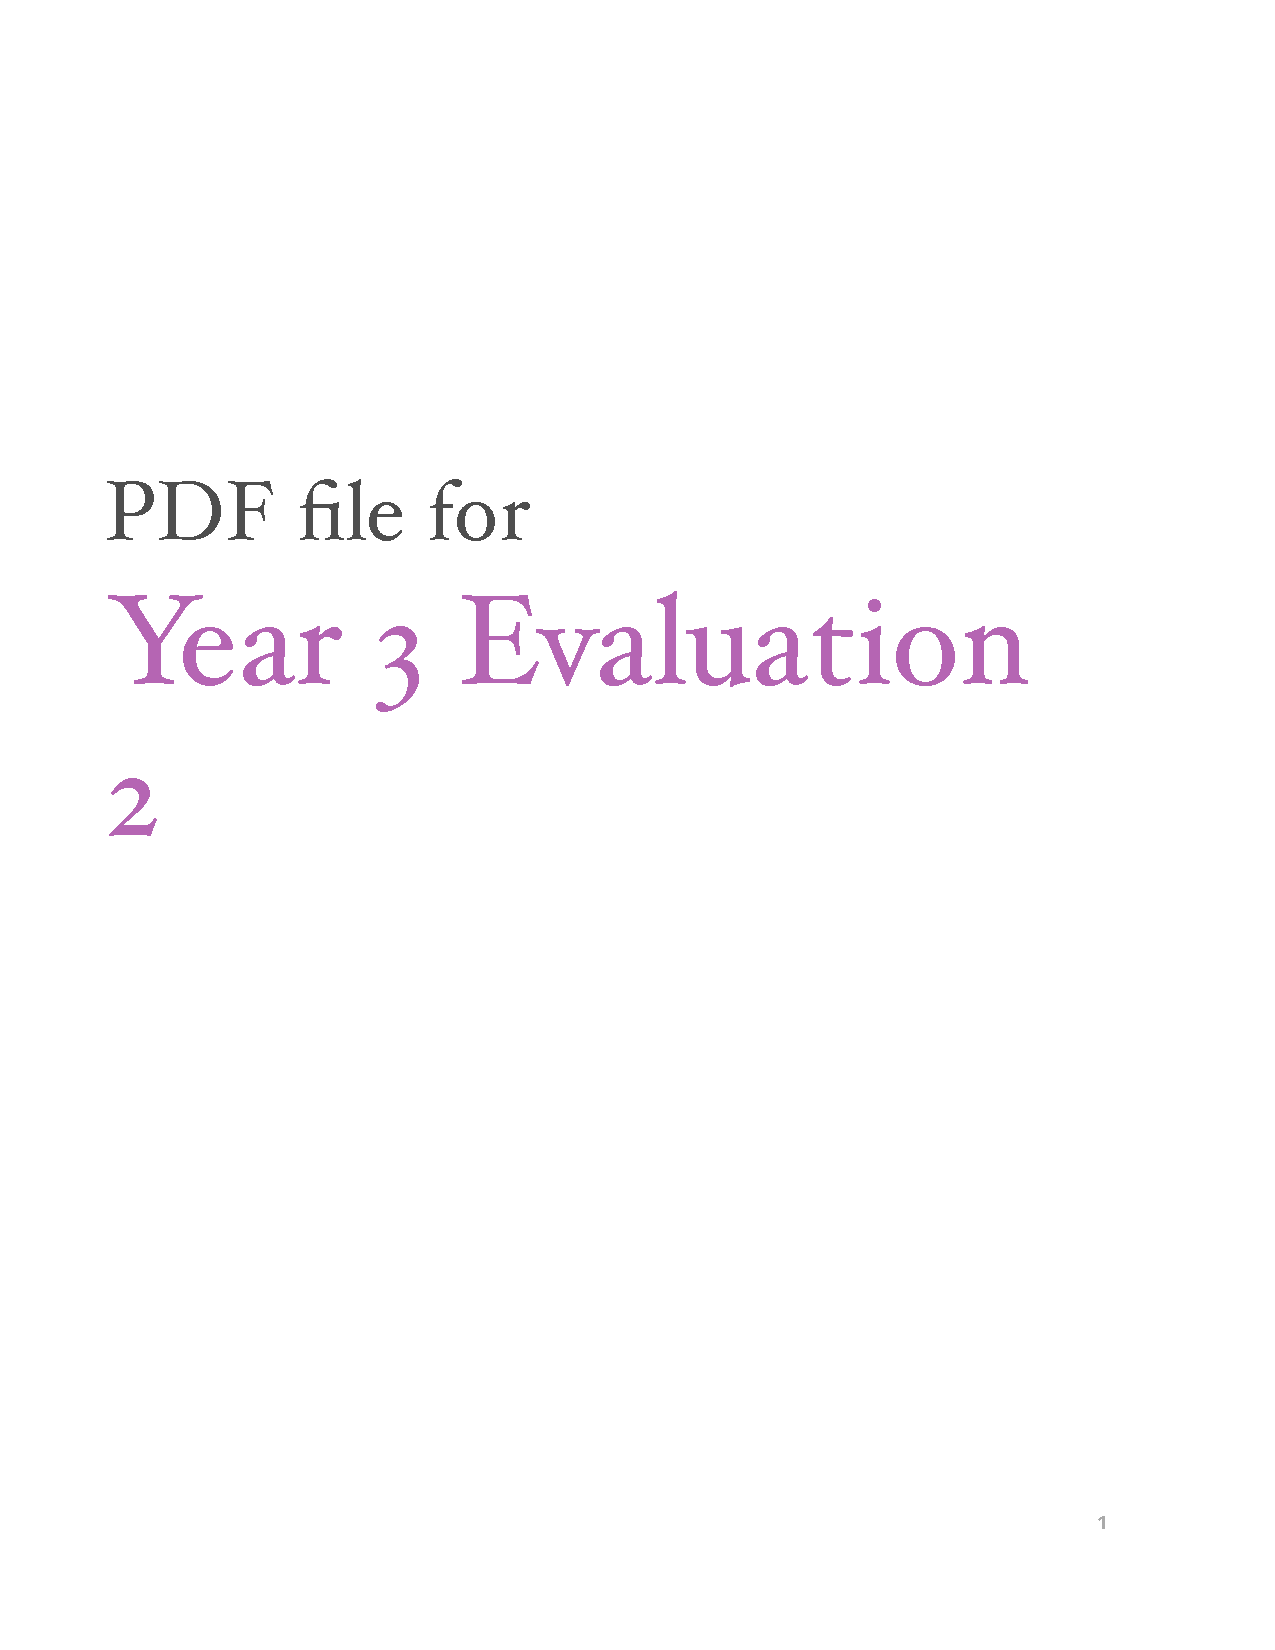
\includepdf[scale=0.9,pages=1-,pagecommand={},angle=0]{Files/7_Evidence_in_Support_of_Effective_Teaching/Evaluations/Y3/Evaluation2.pdf}

\newpage
\sectiontitle{8.) Publications/Creative Achievement}
\fakesection{Publications/Creative Achievement}
\label{Publications}

%Candidates should document their peer-reviewed publications and/or creative achievements in their field.
%(A). Research Publications. List academic publications according to the following categories: Refereed Journals, Books, and Other. Other may include chapters in edited collections, proceedings of meetings, edited texts. Document your publications with reviews of your work, letters of acceptance from editors, photocopies of title pages, the first few pages of the article, etc. In cases of multiple authorship, a narrative description (approx. 250 words or less) of the candidate’s intellectual contribution is required. Do not include self-published works or non-academic publications in this category.
%For promotion, accomplishments since coming to CSU are of far greater importance than achievements at another institution.
%(B). Creative achievements pertinent to the candidate’s professional focus. List creative achievements, including the following categories: artwork, collections, compositions, curated exhibits, exhibited artwork, art and graphic design commissions, moving image, multimedia/databases/websites, radio & television, music recitals & theatrical performances, recordings, juried shows, creative writing readings. Indicate whether each work was juried, invited, reproduced, cited/reviewed in publications, and whether each work was international, national, regional/state, or local in scope.
%The creative production and professional work in fields such as fine and performing arts should be accepted as equivalent to scholarly publication or research.
%(C). Other New or Innovative Scholarly Achievements. Candidates should document other, not easily categorized scholarly achievements.
%Examples include publication of an annotated review of literature on a topic relevant to teaching or research discipline; publication of analysis of data collected on new teaching methods, or evidence of adoption by peers of a mentoring or teaching process developed by the candidate.



\begin{table}[H]
\centering
%\captionof{table}{}
\label{Publications_total}
\begin{tcolorbox}[colback=yellow!10!white,colframe=csuOrange,title=\caption{Total number of published articles by Dr. X in peer-reviewed journals.}]
\begin{tcolorbox}[tab2,tabularx={c}]
{\bf From joining University NAME (2016--2020)} \\
 \toprule
%
\begin{tabularx}{.98\linewidth}{ l|c }
%  \toprule
%\multicolumn{2}{c}{Central State University (2016--2020)} \\
Publication Type & \# of Publications    \\
 \specialrule{1.5pt}{1pt}{1pt}
Original Research Paper &  X  \\
Conference Paper &  Y  \\
Comment Paper &   Z \\
\hline
 Total: & X+Y+Z \\
\end{tabularx}
\\
\bottomrule
\end{tcolorbox}

\begin{tcolorbox}[tab2,tabularx={c}]
{\bf Before joining University NAME (2007--2016)} \\
 \toprule
%
\begin{tabularx}{.98\linewidth}{ l|c }
%  \toprule
%\multicolumn{2}{c}{Central State University (2016--2020)} \\
Publication Type & \# of Publications    \\
 \specialrule{1.5pt}{1pt}{1pt}
Original Research Paper &  X  \\
Conference Paper &  Y  \\
Comment Paper &   Z \\
\hline
 Total: & X+Y+Z \\
\end{tabularx}
 \\
\bottomrule
\end{tcolorbox}

\end{tcolorbox}

\end{table}


\newpage

 \subsection{Publications from joining University NAME (2016 -- 2020)}

\begin{enumerate}
  \itemsep-0.3em
  \item[]

\hskip-1cm \quad\faCaretRight~ {\bf \color{csuOrange} Peer-Reviewed Journal Articles}


\vskip.5em
\item  \textbf{Author 1}, Author 2,
Journal Name, Volume (Year).
\href{https://doi.org/DOI}{\textit{Article Title.}}


\vskip.5em
\hskip-1cm \quad\faCaretRight~ {\bf \color{csuOrange} Peer-Reviewed Conference Proceedings}

\vskip.5em
\item  \textbf{Author 1}, Author 2,
Journal Name, Volume (Year).
\href{https://doi.org/DOI}{\textit{Article Title.}}


\vskip.5em
\hskip-1cm \quad\faCaretRight~ {\bf \color{csuOrange} Peer-Reviewed Comments}

\vskip.5em
\item  \textbf{Author 1}, Author 2,
Journal Name, Volume (Year).
\href{https://doi.org/DOI}{\textit{Article Title.}}

\end{enumerate}

\subsection{Publications before joining University NAME}

\begin{enumerate}
  \itemsep-0.3em
  \item[]

\hskip-1cm \quad\faCaretRight~ {\bf \color{csuOrange} Peer-Reviewed Journal Articles}


\vskip.5em
\item  \textbf{Author 1}, Author 2,
Journal Name, Volume (Year).
\href{https://doi.org/DOI}{\textit{Article Title.}}


\vskip.5em
\hskip-1cm \quad\faCaretRight~ {\bf \color{csuOrange} Peer-Reviewed Conference Proceedings}

\vskip.5em
\item  \textbf{Author 1}, Author 2,
Journal Name, Volume (Year).
\href{https://doi.org/DOI}{\textit{Article Title.}}


\vskip.5em
\hskip-1cm \quad\faCaretRight~ {\bf \color{csuOrange} Peer-Reviewed Comments}

\vskip.5em
\item  \textbf{Author 1}, Author 2,
Journal Name, Volume (Year).
\href{https://doi.org/DOI}{\textit{Article Title.}}

\end{enumerate}

A copy of Dr. X's publications (Y articles) from joining University NAME is enclosed in the following pages.


\includepdf[scale=0.9,pages=1-,pagecommand={}]{Files/8_Papers/Article1.pdf}

\includepdf[scale=0.9,pages=1-,pagecommand={}]{Files/8_Papers/Article2.pdf}

\newpage
\sectiontitledouble{9.) Recognition of Other}{Scholarly Activities}
\fakesection{Recognition of Other Scholarly Activities}
\label{Recognition_Other_Scholarly_Activities}

%Candidates should document other scholarly achievements in this section. Grants/contracts, self-published materials, and research printed in non-refereed or on- campus publications should be included here. Candidates should be specific and not duplicate items in section 8.
%Research and Hybrid faculty should label work approved by the Land Grant Director or designee as “LG approved.”
%Examples of items belonging in this section include, but are not limited to:
%(A). Grants and Contracts. Include external grants received and provide information regarding your role (Principal writer, co-investigator, etc.), the granting or contracting agency, amount requested, and amount funded.
%(B). Scholarly Presentations. List scholarly presentations given during review period. Include keynote addresses, papers, posters, or workshops presented at academic conferences or in settings that may call for more applied scholarship (business, industry, community, etc.). Provide specific information about dates, titles, the nature of the conference (international, national, state, regional/state, or local) and the nature of the presentation. Include names of co-authors and whether presentation was invited or refereed.
%(C). Scholarly Participation at Conferences/Professional Meetings. List the events at professional meetings in which you have had an official role, other than presenting your own scholarship. For example—organizing a conference, developing and chairing a session, serving as an invited respondent to others’ scholarship, or participating in a panel discussion. Clarify the nature of your role, the nature of the meeting (international, national, regional, etc.), and the ways your participation was scholarly.
%(D). Meeting/Conferences Attended. List conferences, workshops, or other professional activities you attended within the review period. Be specific about the organization, location, and date of each meeting and whether it was international, national, regional, state, or local.
%(E). Professional Memberships/Affiliations. List any organizations to which you belong and in which you participate in a scholarly way (fulfill a role beyond paying your annual dues). Give name(s) of the organization(s), the dates of your membership (within the review period), and a brief explanation of the way this membership has influenced your scholarship.
%(F). Professional Licenses. List any current Professional Licenses you have received from professional organizations and explain how these have enhanced your ability to positively affect students in your courses and enhance the image of the institution.
%(G). Editing. List any professional service as journal editor, editorial reviewer for journals or other learned publications.
%(H). Other Evidence and Recognition of Scholarly Contributions. Describe any aspects of your professional growth during the review period that do not fit into the above categories but that warrant consideration for fulfillment of the research/creative achievement requirements for tenure or promotion.


\frame{
%\textbf{Heighlights:}
%
\quad\faCaretRight~ \textbf{External Grant:} (Year-Year) Agency NAME (\$XYZ)

\quad\faCaretRight~ \textbf{Conference Presentations:}
X presentations (T talks, P posters, S seminars, and I invited talks). From joining University NAME, T2 talks in Conference LIST CONFERENCE NAME, and the co-author of I2 papers presented in international conferences in LIST INTERNATIONAL CONFERENCE NAME.

\quad\faCaretRight~ \textbf{Serving on the Editorial Board of X Peer-Reviewed Journals.}

\quad\faCaretRight~ \textbf{Professional and Faculty Development Workshops:}
Participated in Y (Z from joining University NAME) professional and faculty development conferences and workshops.


\quad\faCaretRight~ \textbf{International Conference Organization:}
Served on the international advisory committee of Conference NAME.

}


\newpage
\subsection{Grants}


\blindtext

\frame{
\begin{itemize}
\item \textbf{Project Title:} PROJECT TITLE
\item \textbf{Role:} Sole Principle Investigator
\item \textbf{Award Amount:} \$X
\item \textbf{Date submitted:} DATE
\item \textbf{Date Awarded:} DATE
\end{itemize}
}
%I am the Principle Investigator of a proposal funded by the National Science Foundation’s HBCU-UP/Excellence in Research Program in July 2020.




\begin{description}
\item[Project Overview]
\blindtext

\item[Intellectual Merit]
\blindtext

\item[Broader Impacts of the Project]
\blindtext

\end{description}

\begin{figure*}[h]
\caption{The details of the Award from AGENCY'S NAME website.}
\centering
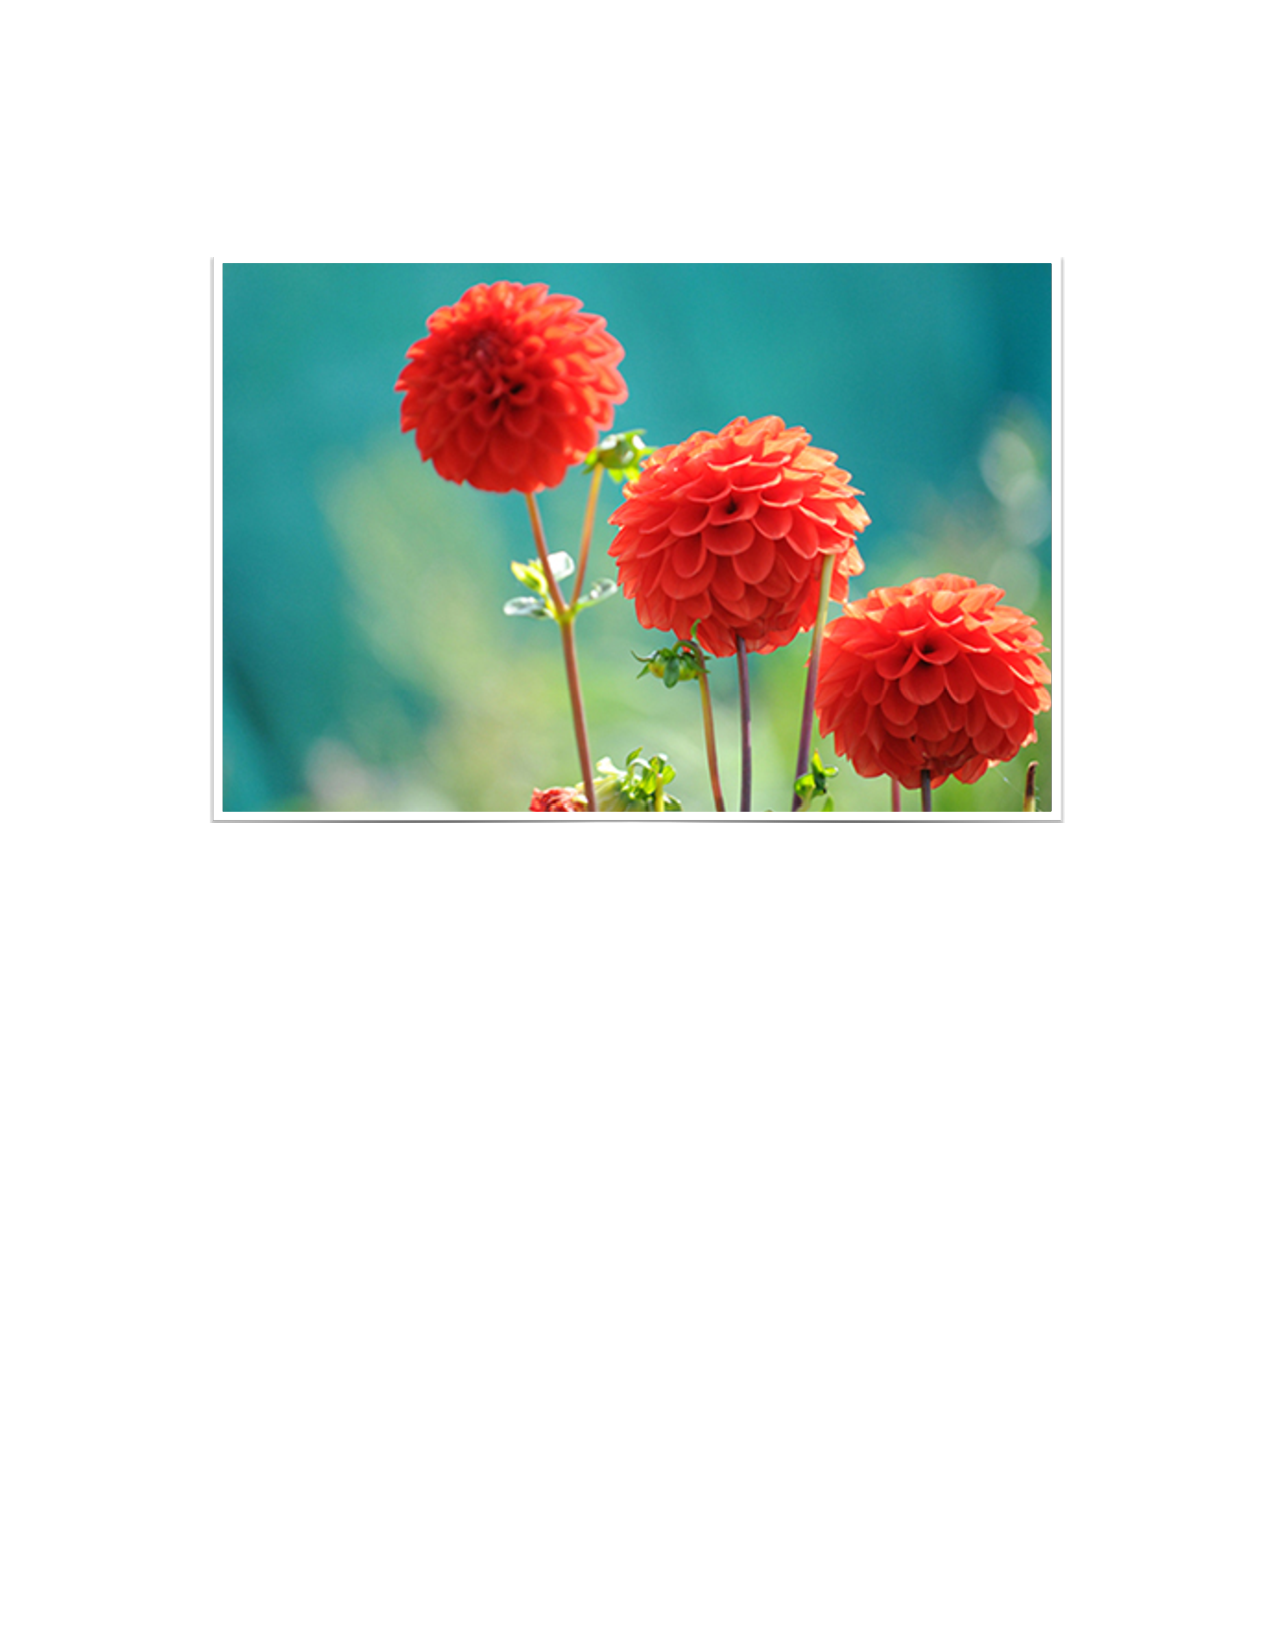
\includegraphics[width=0.75\textwidth]{Files/9_Grants_Presentations/Award_notice.pdf}
\end{figure*}



%\includepdf[scale=0.9,pages=1,pagecommand={}]{Files/9_Grants_Presentations/NSF_EiR}


\newpage
\subsection{Scholarly Presentations}
\begin{enumerate}
\itemsep-0.7em
\item[]

{\item \textbf{Author 1}, Author 2,
\href{http://meetings_address}{Conference NAME}, LOCATION, DATA.
\textit{\href{http://presentation_address}{Presentation TITLE}} (talk)}
\vskip.5em
%
{\item \textbf{Author 1}, Author 2,
\href{http://meetings_address}{Conference NAME}, LOCATION, DATA.
\textit{\href{http://presentation_address}{Presentation TITLE}} (poster)}
\vskip.5em


%\end{enumerate}
\end{enumerate}


The abstracts of the first X presentations, related to the evaluation period of YEAR to YEAR, are enclosed in the following pages.

\newpage


\includepdf[scale=0.9,pages=1,pagecommand={}]{Files/9_Grants_Presentations/Conferences/Abstract1.pdf}


\includepdf[scale=0.9,pages=1,pagecommand={}]{Files/9_Grants_Presentations/Conferences/Abstract2.pdf}



\newpage
\subsection{Scholarly Participation at Conferences/Professional Meetings}
\begin{itemize}
\item {}{Member of International Advisory Committee for \href{https://Conference_address}{"Conference NAME"}, LOCATION, DATE.}

\item Conference Website: \href{http://Conference-address}{http://Conference-address}

\item Conference Proceedings: Journal NAME, \\
\href{https://Journal-address}{https://Journal-address}
\end{itemize}

Please see the list of the {\it International Advisory Committee} on the X page of the enclosed file.

\newpage


\includepdf[scale=0.9,pages=1-,pagecommand={}]{Files/9_Grants_Presentations/Conferences/Conference_Advisory.pdf}


\newpage
\subsection{Meeting/Conferences Attended}

\begin{itemize}

\item{DATE}{\quad \href{https://conference-address}{Conference NAME}}{}{}{}{}

\item{DATE}{\quad \href{https://conference-address}{Conference NAME}}{}{}{}{}


\end{itemize}




\newpage
\subsection{Professional Memberships/Affiliations}

\begin{itemize}

\item {DATE:\quad}{Organization NAME \href{http://Organization-address/}{(Organization NAME)}, ADDRESS.}

\item {DATE:\quad}{Organization NAME \href{http://Organization-address/}{(Organization NAME)}, ADDRESS.}

\end{itemize}


%\newpage
\subsection{Editing}

\begin{itemize}

\item {DARE:\quad}{Member of the editorial board of \href{https://journal-address}{Journal NAME}.}

\item {DARE:\quad}{Member of the editorial board of \href{https://journal-address}{Journal NAME}.}



\vskip1.em
The evidence of serving on the editorial board of the mentioned journals is enclosed in the following pages.


\includepdf[scale=0.9,pages=1,pagecommand={}]{Files/9_Grants_Presentations/Editorial/journal1}


\includepdf[scale=0.9,pages=1,pagecommand={}]{Files/9_Grants_Presentations/Editorial/journal2}

\end{itemize}

\newpage
\sectiontitledouble{10.) Research/Creative/Professional}{Work in Progress}
\fakesection{Research/Creative/Professional Work in Progress}

%Briefly describe your work in progress. Include the focus of your research, scholarly or creative work, major accomplishments, and plans for the future.. Photocopies of up to 10 pages of written work may be included.

\newpage


I am currently working on the following projects ...

\begin{enumerate}

\item {\bf PROJECT 1}
\blindtext

\item {\bf PROJECT 2}
\blindtext

\end{enumerate}

\addtocontents{toc}{\protect\newpage}
\addtocontents{toc}{\protect\thispagestyle{empty}}
\newpage
\sectiontitle{11.) University and Professional Service}
\fakesection{University and Professional Service}
\label{University_Professional_Service}

%(A). University Service. University service is defined as all University committee assignments and any other service assignments in which you serve as a representative of the Central State University’s faculty. These include, but are not limited to, standing and ad hoc committees of the University, the University Senate, CSU-AAUP, college and department standing and ad hoc committees; extension activities; University administrative positions (Department Chairperson, President of the Faculty Senate, director of a program, etc.); and advisor to a student organization. (B). Professional service. Professional service is characterized by those activities conducted both on behalf of the University and/or service to professional organizations in the candidate’s academic field and the scholarship of teaching and learning. Some examples of professional service include serving as a reviewer for a journal or other professional organization, serving on advisory or editorial committees for professional associations, serving as a member or officer in a professional organization, organizing a conference or professional workshop, or chairing or responding to a conference panel.


\frame{

\quad\faCaretRight~ \textbf{DATE--DATE:}
Served on {\it University Committee NAME} (DATE: POSITION)

\quad\faCaretRight~ \textbf{DATE--DATE:}
Served on {\it University Committee NAME} (DATE: POSITION)

}



\newpage
\subsection{University Service}
{\bf University Committee NAME (DATE)} \\
\blindtext
%

{\bf University Committee NAME (DATE)} \\
\blindtext \\

A letter from Dr. Y, chair of {\it University Committee NAME}, for my service to this Committee is enclosed in the following pages.


\includepdf[scale=0.9,pages=1-,pagecommand={}]{Files/11_University_Professional_Service/Service_support_letter.pdf}


\subsection{Professional Service}
\label{Professional_Service}

During the course of the evaluation, from DATE to DATE, I reviewed X articles for peer-reviewed journals and wrote Y reports, as some of the papers had more than one round of review.
%
The list of the journals I was invited to review a manuscript for them, in impact factor order, is:
\begin{itemize}
\item \href{https://journal1-address/}{Journal 1} (J1) [1 paper]
\item \href{https://journal2-address/}{Journal 1} (J2) [2 papers]
\end{itemize}
%

The complete list of the verified reviews, including the date of reviews, the title of the articles and journals, prepared by the Publons website, is enclosed in the following pages.


\includepdf[scale=0.9,pages=1-,pagecommand={},angle=0]{Files/11_University_Professional_Service/Publons_verified_eviews.pdf}

\newpage
\sectiontitle{12.) Public Service}
\fakesection{Public Service}
\label{Public_Service}

%Include participation in the activities and institutions of the community on any level. For each performance of service, state offices held; identify the community group or organization with which you are working; provide the length of your service and nature of organization; and explain your role and/or office within the group or organization.

\frame{
\begin{itemize}
\item \textbf{Organization Title:} Organization NAME
\item \textbf{Role:} ROLE
\item \textbf{Period of Service:} DATE
\item \textbf{Website:} \href{https://Organization-address}{https://Organization-address}
\end{itemize}
}

\newpage

\blindtext

\vskip1cm
A declaration letter from X, Director of Organization NAME, for my service to Y is enclosed in the following page.


\includepdf[scale=0.9,pages=1-,pagecommand={},angle=0]{Files/12_Public_Service/support_Letter}

\newpage
\sectiontitledouble{13.) Letters from Faculty}{at University NAME}
\fakesection{Letters from Faculty at University NAME}

%These letters should be based on the writer’s first- hand experience with the candidate in the area of teaching, research, and/or service. For example, a letter from a colleague in support of teaching could be based on classroom observations or the respondent’s analysis of the quality and creativity of instructional materials designed by the candidate. Letters from colleagues who hold at least the rank for which you are applying are encouraged.

\frame{
\textbf{Enclosed Letters of Supports}


\begin{itemize}
%\item {\bf Jeremy Holtgrave}, Associate Professor of Physics.
%\item[] [Evaluation of teaching (physics courses), reserach, and service.]

\item {\bf X1 Y1}, POSITION.
\item[] [Evaluation of research.]

\item {\bf X2 Y2}, POSITION.
\item[] [Former chair of Z; Evaluation of teaching, research, and service.]

\end{itemize}

}




\newpage


\includepdf[scale=0.9,pages=1-,pagecommand={}]{Files/13_Internal_Recommendations/Recommendation1}

\includepdf[scale=0.9,pages=1-,pagecommand={}]{Files/13_Internal_Recommendations/Recommendation2}

\newpage
\sectiontitledouble{14.) Scholars and Peers}{Outside of University NAME}
\fakesection{Scholars and Peers Outside of University NAME}


\frame{
\textbf{Enclosed Letters of Supports}

\begin{itemize}
\item \href{https://professor1-address}{X1 Y1}, POSITION, AFFILIATION.
\item \href{https://professor1-address}{X2 Y2}, POSITION, AFFILIATION.
\end{itemize}

}

%Peers from outside of Central State University providing letters of support should possess knowledge of your most recent teaching, research, and/or service accomplishments. Letters from peers may address both professional and personal traits that affirm you as a teacher, advisor, and mentor of students. Letters from peers may be used to comment on any knowledge that the peer may have of your contributions to your discipline in terms of research/publications, creative work, technical reports and professional panel participations. The letters need to include the correspondent’s current institutional information (e.g. their institutional affiliation, rank, position held, etc.). If the peer does not provide such information, please supply that information to the committee.

\newpage


\includepdf[scale=0.9,pages=1-,pagecommand={}]{Files/14_External_Recommendations/Recommendation1}

\includepdf[scale=0.9,pages=1-,pagecommand={}]{Files/14_External_Recommendations/Recommendation2}


\end{document}

